\documentclass[12pt,t]{beamer}
\usepackage{graphicx}
\setbeameroption{hide notes}
\setbeamertemplate{note page}[plain]

% get rid of junk
\usetheme{default}
\beamertemplatenavigationsymbolsempty
\hypersetup{pdfpagemode=UseNone} % don't show bookmarks on initial view

\usepackage{mathtools}
\usepackage{colortbl}
\usepackage{pgf}
\usepackage{pgfkeys}
\usepackage{tikz}
\usetikzlibrary{fpu}

% font
\usepackage{fontspec}
\setsansfont{TeX Gyre Heros}
\setbeamerfont{note page}{family*=pplx,size=\footnotesize} % Palatino for notes
% "TeX Gyre Heros can be used as a replacement for Helvetica"
% In Unix, unzip the following into ~/.fonts
% In Mac, unzip it, double-click the .otf files, and install using "FontBook"
%   http://www.gust.org.pl/projects/e-foundry/tex-gyre/heros/qhv2.004otf.zip

% named colors
\definecolor{offwhite}{RGB}{249,242,215}
% \definecolor{foreground}{RGB}{255,255,255}
\definecolor{foreground}{RGB}{0,0,0}
% \definecolor{background}{RGB}{24,24,24}
\definecolor{background}{RGB}{255,255,255}
\definecolor{title}{RGB}{107,174,214}
\definecolor{gray}{RGB}{100,100,100}
\definecolor{subtitle}{RGB}{102,255,204}
\definecolor{hilight}{RGB}{20,180,204}
\definecolor{vhilight}{RGB}{255,111,207}
\definecolor{lolight}{RGB}{155,155,155}
%\definecolor{green}{RGB}{125,250,125}


% use those colors
\setbeamercolor{titlelike}{fg=title}
\setbeamercolor{subtitle}{fg=title}
\setbeamercolor{institute}{fg=gray}
\setbeamercolor{normal text}{fg=foreground,bg=background}
\setbeamercolor{item}{fg=foreground} % color of bullets
\setbeamercolor{subitem}{fg=gray}
\setbeamercolor{itemize/enumerate subbody}{fg=gray}
\setbeamertemplate{itemize subitem}{{\textendash}}
\setbeamerfont{itemize/enumerate subbody}{size=\footnotesize}
\setbeamerfont{itemize/enumerate subitem}{size=\footnotesize}


% settings for table of contents
\setbeamercolor{section in toc}{fg=foreground,bg=background}
\setbeamerfont{subsection in toc}{size=\footnotesize}
\setbeamertemplate{section in toc}{{\scriptsize\leavevmode\raise1.35pt\hbox{$\blacktriangleright$}} \inserttocsection}
%\setbeamertemplate{subsection in toc}{\quad{\tiny\leavevmode\raise1.5pt\hbox{$\blacktriangleright$}} \footnotesize\inserttocsubsection\\}
\setbeamertemplate{subsection in toc}{\quad\quad\textendash\enspace\inserttocsubsection\\}

% page number
\setbeamertemplate{footline}{%
    \raisebox{5pt}{\makebox[\paperwidth]{\hfill\makebox[20pt]{\color{gray}
          \scriptsize\insertframenumber}}}\hspace*{5pt}}


% add a bit of space at the top of the notes page
\addtobeamertemplate{note page}{\setlength{\parskip}{12pt}}

% add subsection as frame title when it is empty
\makeatletter
  \CheckCommand*\beamer@checkframetitle{%
    \@ifnextchar\bgroup\beamer@inlineframetitle{}}
  \renewcommand*\beamer@checkframetitle{%
    \global\let\beamer@frametitle\relax\@ifnextchar%
    \bgroup\beamer@inlineframetitle{}}
\makeatother

\addtobeamertemplate{frametitle}{
  \ifx\insertframetitle\empty
      \frametitle{\insertsubsectionhead}
  \else
  \fi
 }{}

% for colored cells in tabular
\usepackage{colortbl}

% a few macros
\newcommand{\bi}{\begin{itemize}}
\newcommand{\ei}{\end{itemize}}
\newcommand{\ig}{\includegraphics}
\newcommand{\subt}[1]{{\footnotesize \color{subtitle} {#1}}}


% title info
\title{Mathematics}
%\subtitle{Part 2}
\author{Tómas Ken Magnússon \\Bjarki Ágúst Guðmundsson}
\institute{\href{http://ru.is/td}{School of Computer Science} \\[2pt] \href{http://ru.is}{Reykjavík University}}
\date{Árangursrík forritun og lausn verkefna}
% \date{\href{http://www.biostat.wisc.edu/~kbroman}{\tt \scriptsize biostat.wisc.edu/{\textasciitilde}kbroman}
% \\[-4pt]
% \href{http://github.com/kbroman}{\tt \scriptsize github.com/kbroman}
% }


% Tikz
\usepackage{tikz}
\usetikzlibrary{arrows,shapes}

% minted
\usepackage{minted}
\usemintedstyle{tango}
\newminted{cpp}{fontsize=\footnotesize}
\newminted{cppsmall}{fontsize=\scriptsize}

% Graph styles
\tikzstyle{vertex}=[circle,fill=black!50,minimum size=15pt,inner sep=0pt, font=\small]
\tikzstyle{selected vertex} = [vertex, fill=red!24]
\tikzstyle{edge} = [draw,thick,-]
\tikzstyle{dedge} = [draw,thick,->]
\tikzstyle{weight} = [font=\scriptsize,pos=0.5]
\tikzstyle{selected edge} = [draw,line width=2pt,-,red!50]
\tikzstyle{ignored edge} = [draw,line width=5pt,-,black!20]

\def\hepta{\draw[foreground](A) -- (B) -- (C) -- (D) -- (E) -- (F) -- (G) -- cycle;}

% Macro for drawing polygon diagonals. 
% Example \slice{A/C,C/E,E/G,C/G}

\newcommand{\slice}[1]{%
    \hepta
    \draw[foreground] \foreach \x/\y in {#1} {(\x)--(\y)};
}

\AtBeginSection[]
{
  \begin{frame}<beamer>{Mathematics}
    \vspace{20pt}
    \tableofcontents[
      currentsection,
      hideallsubsections,
      %currentsubsection,
      %hideothersubsections,
      sectionstyle=show/shaded%,
      %subsectionstyle=show/shaded/hide
    ]
  \end{frame}
}

\begin{document}

% title slide
{
    \setbeamertemplate{footline}{} % no page number here
    \frame{
        \titlepage
    }
}

\begin{frame}{Today we're going to cover}
    \vspace{22pt}
    %\bi
      %\item Basics
      %\item Number Theory
      %\item Combinatorics
      %\item Game Theory
      %\item Probability Theory
      %\item BigInteger
      %\item Applications
    %\ei
    \tableofcontents[hideallsubsections]
\end{frame}

%%%%% BASICS %%%%%%%%%%%%%%%%%%%%%%%%%%%%%%%%%%%%%%%%%%%%%%%%%%%%%%%%%%%%%
\section{Basics}
\subsection{General overview}
%\begin{frame}{Basics}
  %\vspace{40pt}
  %\bi
    %\item General overview
    %\item Finding patterns, formulas
    %\item Arithmetic/geometric progression
    %\item Using logarithm
    %\item Base conversion
    %\item Working with doubles, epsilon
  %\ei
%\end{frame}

\begin{frame}%{General overview}
  \vspace{60pt}
  \begin{center}
  Computer Science $\subset$ Mathematics
  \end{center}
    %\item Usually in competitions there is at least one problem that involves
      %solving mathematically before coding.
\end{frame}

\begin{frame}
  \vspace{40pt}
  \bi
    %\item Usually in competitions there is at least one problem that involves
      %solving mathematically before coding.
    \item Usually at least one problem that involves solving mathematically.
    %\item Problems often require mathematics to simplify problems so they can
      %be solved efficiently, overlapping other problem solving paradigms.
    \item Problems often require mathematical analysis to be solved efficiently.
    \item Using a bit of math before coding can also shorten and simplify code.
  \ei
\end{frame}

\subsection{Finding patterns and formulas}

\begin{frame}
  \vspace{20pt}
  \bi
    % TODO: What is it really?
    \item Some problems have solutions that form a pattern.
    \onslide<2-> \item By finding the pattern, we solve the problem.
    \item Could be classified as mathematical ad-hoc problem.
    \item Requires mathematical intuition.
    \onslide<3->{
      \item Useful tricks:
        \bi
          \item Solve some small instances by hand.
          \item See if the solutions form a pattern.
        \ei
    } \onslide<4-> {
      \item Does the pattern involve some overlapping subproblem?
    } \onslide<5-> {
        We might need to use {\color{vhilight}DP}.
    } \onslide<6-> {
      \item Knowing reoccurring identities and sequences can be helpful.
    }
  \ei
\end{frame}

%\begin{frame}[fragile]{Example}
  %Let's see an example
  %% TODO: Example
%\end{frame}

\subsection{Arithmetic and geometric progression}

\begin{frame}{Arithmetic progression}
  \vspace{30pt}
  \bi
    \item Often we see a pattern like
      \[
        2 , 5 , 8 , 11 , 14, 17, 20, \ldots
      \]
    \onslide<2->
    \item This is called a arithmetic progression.
      \[
        a_n = a_{n-1} + c
      \]
  \ei
\end{frame}

\begin{frame}{Arithmetic progression}
  \vspace{30pt}
  \bi
    \item Depending on the situation we may want to get the $n$-th element
      \[
        a_n = a_1 + (n-1) c
      \]
    \item Or the sum over a finite portion of the progression
      \[
        S_n = \frac{n(a_1 + a_n)}{2}
      \]
    \onslide<2->
    \item Remember this one?
      \[
        1 + 2 + 3 + 4 + 5 + \ldots + n = \frac{n(n+1)}{2}
      \]
  \ei
\end{frame}

\begin{frame}{Geometric progression}
  \vspace{30pt}
  \bi
    \item Other types of pattern we often see are geometric progressions
      \[
        1,\, 2,\, 4,\, 8,\, 16,\, 32,\, 64,\, 128,\, \ldots
      \]
    \onslide<2->{
      \item More generally
        \[
          a,\, ar,\, ar^2,\, ar^3,\, ar^4,\, ar^5,\, ar^6,\, \ldots
        \]
        \[
          a_n  = a r^{n-1}
        \]
      }
  \ei
\end{frame}

\begin{frame}{Geometric progression}
  \vspace{30pt}
  \bi
    \item Sum over a finite portion
      \[
        \sum_{i = 0}^n ar^i =  \frac{a(1-r^n)}{(1-r)}
      \]
    \onslide<2->{
      \item Or from the $m$-th element to the $n$-th
        \[
          \sum_{i = m}^n ar^i =  \frac{a(r^{m}-r^{n+1})}{(1-r)}
        \]
    }
  \ei
\end{frame}

\subsection{Little bit about logarithm}
\begin{frame}[fragile]
  \vspace{30pt}
  \bi
    \item Sometimes doing computation in logarithm can be an efficient alternative.

    \onslide<2->
  \item In both C++(\texttt{\color{gray}<cmath>}) and
    Java(\texttt{\color{gray}java.lang.Math}) we have the natural logarithm
    %we have from \texttt{\color{gray}<cmath>} the natural logarithm
      \begin{minted}{cpp}
    double log(double x);
      \end{minted}

    \onslide<3->
      and logarithm in base $10$
      \begin{minted}{cpp}
    double log10(double x);
      \end{minted}
    \onslide<4->
  \item And also the exponential
    \begin{minted}{cpp}
    double exp(double x);
    \end{minted}
  \ei
\end{frame}

\begin{frame}[fragile]{Example}
  \vspace{20pt}
  \bi
    \item For example, what is the first power of $17$ that has $k$ digits in base $b$?
    \onslide<2->
    \item {\color{title}Naive solution}: Iterate over powers of $17$ and count the number of digits.
    \onslide<3->
    \item But the powers of $17$ grow exponentially!
      \[17^{16} > 2^{64}\]
    \item What if $k = 500$ ($\sim1.7 \cdot 10^{615}$), or something larger?
    \onslide<4->
    \item Impossible to work with the numbers in a normal fashion.
    \item Why not $\log$?
  \ei
\end{frame}

\begin{frame}[fragile]{Example}
  \vspace{40pt}
  \bi
    \item Remember, we can calculate the length of a number $n$ in base $b$
      with $\lfloor \log_b(n) \rfloor + 1$.
    \onslide<2->
    \item But how do we do this with only $\ln$ or $\log_{10}$?
    \onslide<3->
    \item Change base!
      \[
        \log_b(a) = \frac{\log_d(a)}{\log_d(b)} = \frac{\ln(a)}{\ln(b)}
      \]
    \item Now we can at least count the length without converting bases
      %\begin{minted}{cpp}
%int digitsInBase(int n, int b){
  %return static_cast<int>(floor(log(n)/log(b)) + 1);
%}
      %\end{minted}
  \ei
\end{frame}

\begin{frame}{Example}
  \vspace{20pt}
  \bi
    \item We still have to iterate over the powers of $17$, but we can do that in log
      \[
        \ln(17^{x-1} \cdot 17) = \ln(17^{x-1}) + \ln(17)
      \]
    \onslide<2->
    \item More generally
      \[
        \log_b(xy) = \log_b(x) + \log_b(y)
      \]
    \item For division
      \[
        \log_b(\frac{x}{y}) = \log_b(x) - \log_b(y)
      \]
  \ei
\end{frame}

\begin{frame}{Example}
  \vspace{20pt}
  \bi
    \item We can simplify this even more.
    \item The solution to our problem is in mathematical terms, finding the $x$ for
      \[
        \log_b(17^x) = k - 1
      \]
    \onslide<2->
    \item One more handy identity
      \[
        \log_b(a^c) = c \cdot \log_b(a)
      \]
    \onslide<3->
    \item Using this identity and the ones we've covered, we get
      \[
        x = \left\lceil (k-1) \cdot \frac{\ln(10)}{\ln(17)} \right\rceil
      \]
  \ei
\end{frame}

\subsection{Base conversion}
\begin{frame}[fragile]
  \vspace{20pt}
  \bi
    \item Speaking of bases.
    \onslide<2->
    \item What if we actually need to use base conversion?
    \onslide<3->
    \item Simple algorithm
      \begin{minted}{cpp}
vector<int> toBase(int base, int val) {
    vector<int> res;
    while(val) {
        res.push_back(val % base);
        val /= base;
    }
    return val;
      \end{minted}
    \item Starts from the $0$-th digit, and calculates the multiple of each power.
  \ei
\end{frame}

\subsection{Working with doubles}

\begin{frame}[fragile]
  \vspace{30pt}
  \bi
  \onslide<2->
    \item Comparing doubles, sounds like a bad idea.
  \onslide<3->
    \item What else can we do if we are working with real numbers?
  \onslide<4->
    \item We compare them to a certain degree of precision.
  \onslide<5->
    \item Two numbers are deemed equal of their difference is less than some small epsilon.
  \ei

    \begin{minted}{cpp}
    const double EPS = 1e-9;

    if (abs(a - b) < EPS) {
    ...
    }
    \end{minted}
\end{frame}

\begin{frame}[fragile]
  \vspace{40pt}
  \bi
    \item Less than operator:
      \begin{minted}{cpp}
    if (a < b - EPS) {
    ...
    }
      \end{minted}
    \item Less than or equal:
      \begin{minted}{cpp}
    if (a  < b + EPS) {
    ...
    }
    \end{minted}
    \item The rest of the operators follow.
  \ei
\end{frame}

\begin{frame}[fragile]
  \vspace{30pt}
  \bi
    \item This allows us to use comparison based algorithms.
    \onslide<2->
    \item For example \mintinline{cpp}{std::set<double>}.
      \begin{minted}{cpp}

struct cmp {
    bool operator(){double a, double b}{
        return a < b - EPS;
    }
};

set<double, cmp> doubleSet();
      \end{minted}
    \item Other STL containers can be used in similar fashion.
  \ei
\end{frame}

%%% NUMBER THEORY %%%%%%%%%%%%%%%%%%%%%%%%%%%%%%%%%%%%%%%%%%%%%%%%%%%%

\section{Number Theory}
\subsection{Modular arithmetic}
\begin{frame}[fragile]
  \vspace{40pt}
  \bi
    \item Problem statements often end with the sentence \\
      \vspace{10pt}
      \begin{quote}
``... and output the answer modulo n.''
      \end{quote}
      \vspace{10pt}
  \onslide<2->
    \item This implies that we can do all the computation with integers \emph{modulo }$n$.
  \onslide<3->
    %\item Working with a finite set of numbers
    \item The integers, modulo some $n$ form a structure called a \emph{ring}.
  \onslide<4->
    %\item There are some special rules that apply to modular arithmetic, and also
      %some very interesting properties.
    \item Special rules apply, also loads of interesting properties.
  \ei
\end{frame}

\begin{frame}
  \vspace{20pt}
  Some of the allowed operations:
  \bi
    \item Addition and subtraction modulo $n$
      \begin{align*}
        (a \bmod n) + (b \bmod n) = (a + b \bmod n) \\
        (a \bmod n) - (b \bmod n) = (a - b \bmod n)
      \end{align*}
    \item Multiplication
      \[
        (a \bmod n)(b \bmod n) = (ab \bmod n)
      \]
    \item Exponentiation
      \[
        (a \bmod n)^b = (a^b \bmod n)
      \]
    \item \emph{Note:} We are only working with integers.
  \ei
\end{frame}

\begin{frame}
  \vspace{40pt}
  \bi
    \item What about division? \onslide<2->{{\color{vhilight}NO!}}
  \onslide<3->
    \item We could end up with a fraction!
    \item Division with $k$ equals multiplication with the \emph{multiplicative
      inverse} of $k$.
  \onslide<4->
    \item The \emph{multiplicative inverse} of an integer $a$, is the element $a^{-1}$ such that
      \[
        a \cdot a^{-1} = 1 \pmod{n}
      \]
  \ei
\end{frame}

\begin{frame}
  \vspace{40pt}
  \bi
    \item What about logarithm? \onslide<2->{{\color{hilight}YES!}}
      \onslide<2->
      \bi
        \item But difficult.
        \onslide<3->
        \item Basis for some cryptography such as elliptic curve, Diffie-Hellmann.
      \ei
    \item Google ``Discrete Logarithm'' if you want to know more.
  \ei
\end{frame}

\begin{frame}{Definitions that everybody should know}
  \vspace{15pt}
  \bi
    \item {\color{hilight}Prime number} is a positive integer greater than $1$
      that has no positive divisor other than $1$ and itself.
    \item {\color{hilight}Greatest Common Divisor} of two integers $a$ and $b$ is the
      largest number that divides both $a$ and $b$.
    \item {\color{hilight}Least Common Multiple} of two integers $a$ and $b$ is
      the smallest integer that both $a$ and $b$ divide.
    \item {\color{hilight}Prime factor} of an positive integer is a prime number that divides it.
    \item {\color{hilight}Prime factorization} is the decomposition of an
      integer into its prime factors. By the fundamental theorem of
      arithmetics, every integer greater than $1$ has a unique prime
      factorization.
  \ei
\end{frame}

\begin{frame}[fragile]{Extended Euclidean algorithm}
  \vspace{20pt}
  \framesubtitle{-- and non-extended}
  \bi
    \item The Euclidean algorithm is a recursive algorithm that computes the GCD of two numbers.
      \begin{minted}{cpp}
int gcd(int a, int b){
    return b == 0 ? a : gcd(b, a % b);
}
    \end{minted}
    \item Runs in $O(\log^2 N)$.
    \onslide<2->
    \item Notice that this can also compute LCM
      \[
        \text{lcm}(a, b) = \frac{a\cdot b}{\gcd(a,b)}
      \]
    \item See Wikipedia to see how it works and for proofs.
  \ei
\end{frame}

\begin{frame}[fragile]{Extended Euclidean algorithm}
  \vspace{20pt}
  \bi
    \item Reversing the steps of the Euclidean algorithm we get the B\'ezout's identity
      \[
        \gcd(a, b) = ax + by
      \]
    which simply states that there always exist $x$ and $y$ such that the equation above holds.
    \onslide<2->
    \item The extended Euclidean algorithm computes the GCD and the coefficients $x$ and $y$.
    \item Each iteration it add up how much of $b$ we subtracted from $a$ and vice versa.
  \ei
\end{frame}

\begin{frame}[fragile]{Extended Euclidean algorithm}
  \vspace{10pt}
    \begin{minted}{cpp}
int egcd(int a, int b, int& x, int& y) {
    if (b == 0) {
        x = 1;
        y = 0;
        return a;
    } else {
        int d = egcd(b, a % b, x, y);
        x -= a / b * y;
        swap(x, y);
        return d;
    }
}
    \end{minted}
\end{frame}

\begin{frame}{Applications}
  \vspace{40pt}
  \bi
    \item Essential step in the RSA algorithm.
    \item Essential step in many factorization algorithms.
    \item Can be generalized to other algebraic structures.
    \item Fundamental tool for proofs in number theory.
    \item Many other algorithms for GCD
  \ei
\end{frame}

\subsection{Modular inverse}
\begin{frame}
  \vspace{20pt}
  Back to modular inverse.
  \bi
    \item Working modulo $n$ often requires division (multiplication by inverse).
    \onslide<2->
    \item Given some $a \pmod{n}$, then the multiplicative inverse $a^{-1}
      \pmod{n}$ exists iff. $a$ and $n$ are coprime.
    \onslide<3->
    \item It so happens that when we have from EGCD algorithm
      \[
        ax + ny = \gcd(a,n) = 1
      \]
      then \[ a^{-1} \equiv x \pmod{p} \]
  \ei
\end{frame}

\begin{frame}
  \vspace{20pt}
  \bi
    \item Hence, we have an algorithm to compute modular multiplicative inverse.
      \bi
        \item and it reports if no such element exists, that is $\text{GCD} \neq 1$
      \ei
    \onslide<2->
    \item What if $n$ is a prime number?
    \onslide<3->
    \item Then every element has an inverse.
    \onslide<4->
  \item And we can use Fermat's little theorem
    \[
      a^{p-1} \equiv 1 \pmod{n}
    \]
  \item which implies that
    \[
      a^{p-1}\cdot a^{p-2} \equiv 1 \pmod{n} \quad\Rightarrow\quad a^{-1} = a^{p-2} \pmod{n}
    \]
  \ei
\end{frame}

\begin{frame}
  \vspace{40pt}
  \bi
    \item With $n$ as a prime, the problem of finding the inverse now becomes
      only a matter of exponentiation.
    \onslide<2->
    \item Using the repeated squaring method, we can compute the inverse in $O(\log N)$.
    \onslide<3->
    \item This method only works when working modulo a \textbf{prime}.
  \ei
\end{frame}

\subsection{Chinese remainder theorem}

\begin{frame}
  \vspace{20pt}
  What is the lowest number $n$ such that when divided by
  \vspace{10pt}
  \bi
    \item[] ... $3$ it leaves $2$ in remainder.
    \item[] ... $5$ it leaves $3$ in remainder.
    \item[] ... $7$ it leaves $2$ in remainder.
  \ei
  \vspace{10pt}
  \onslide<2->
  When stated mathematically, find $n$ where
      \begin{align*}
  n &\equiv 2 \pmod{3} \\
  n &\equiv 3 \pmod{5} \\
  n &\equiv 2 \pmod{7}
      \end{align*}
\end{frame}

\begin{frame}
  \vspace{20pt}
  The Chinese remainder theorem states that:
  \bi
    \item When the moduli of a system of linear congruences are pairwise
      coprime, there exists a unique solution modulo the product of the moduli.
  \ei
  \onslide<2->
  Let $n_1, n_2,\ldots, n_k$ be pairwise coprime positive integers, and let $x$
  be the solution to the system of linear congruences
  \begin{align*}
    x &\equiv  b_1 \pmod{n_1} \\
    x &\equiv  b_2 \pmod{n_2} \\
      &\vdots                 \\
    x &\equiv b_k \pmod{n_k}
  \end{align*}
\end{frame}

\begin{frame}
  \vspace{10pt}
  \bi
    \item The Chinese remainder theorem only states that there exists a solution and it
  is unique modulus the product of the moduli. \\
    \item To obtain the solution $x$
      \[
        x \equiv b_1 c_1 \frac{N}{n_1} + \ldots + b_k c_k \frac{N}{n_k}
      \]
      where $N = n_1 n_2 \cdots n_k$.
    \item The coefficients $c_i$ are determined from
      \[
        c_i \frac{N}{n_i} \equiv \pmod{n_i}
      \]
      (the multiplicative inverse of $\frac{N}{n_i}$ modulus $n_i$)
    \item Use EGCD to compute $c_i$.
  \ei
\end{frame}

\subsection{Primality testing}
\begin{frame}
  \vspace{20pt}
  \bi
    \item How do we determine if a number $n$ is a prime?
    \onslide<2->
    \item {\color{title}Naive method:} Iterate over all $1 < i < n$ and check it
      $i \mid n$.
      \bi
        \item  $O(N)$
      \ei
    \onslide<3->
    \item {\color{title}Better:} If $n$ is not a prime, it has a divisor $\leq \sqrt{n}$.
      \bi
        \item Iterate up to $\sqrt{n}$ instead.
        \item $O(\sqrt{N})$
      \ei
    \onslide<4->
    \item {\color{title}Even better:} If $n$ is not a prime, it has a prime divisor $\leq \sqrt{n}$
      \bi
        \item Iterate over the prime numbers up to $\sqrt{n}$.
        \item There are $\sim N/\ln(N)$ primes less $N$, therefore $O(\sqrt{N}/\log N)$.
      \ei
  \ei
\end{frame}

\begin{frame}
  \vspace{40pt}
  \bi
    \item Trial division is a deterministic primality test.
    \item Many algorithms that are probabilistic or randomized.
    \item Fermat test; uses Fermat's little theorem.
    \item Probabilistic algorithms that can only prove that a number is
      composite such as Miller-Rabin.
    \item AKS primality test, the one that proved that primality testing is in
      $P$.
  \ei
\end{frame}

\subsection{Prime sieves}
\begin{frame}[fragile]
  \bi
    \item If we want to generate primes, using a primality test is very inefficient.
    \onslide<2->
    \item Instead, our preferred method of prime generation is the sieve of Eratosthenes.
      \bi
        \onslide<3->
        \item For all numbers from $2$ to $\sqrt{n}$:
        \onslide<4->
        \item If the number is not marked, iterate over every multiple of the
          number up to $n$ and mark them.
        \onslide<5->
        \item The unmarked numbers are those that are not a multiple of any
          smaller number.
        \item $O(\sqrt{N}\log \log N)$
      \ei
  \ei
  \onslide<6->
  \begin{columns}[T]
    \begin{column}{.7\textwidth}
      \centering
      \only<6>{
      \begin{tabular}{|c | c | c | c | c|}
        \hline
        & $2$ & $3$ & $4$ & $5$ \\ \hline
         $6$ & $7$ & $8$ & $9$ & $10$ \\ \hline
         $11 $ & $12$ & $13$ & $14$ & $15$ \\ \hline
         $16$ & $17$ & $18$ & $19$ & $20$ \\ \hline
         $21$ & $22$ & $23$ & $24$ & $25$ \\ \hline
       \end{tabular}}

      \only<7>{
      \begin{tabular}{|c | c | c | c | c|}
        \hline
        & \cellcolor{hilight}$2$ & $3$ & $4$ & $5$ \\ \hline
         $6$ & $7$ & $8$ & $9$ & $10$ \\ \hline
         $11 $ & $12$ & $13$ & $14$ & $15$ \\ \hline
         $16$ & $17$ & $18$ & $19$ & $20$ \\ \hline
         $21$ & $22$ & $23$ & $24$ & $25$ \\ \hline
       \end{tabular}}

      \only<8>{
      \begin{tabular}{|c | c | c | c | c|}
        \hline
        & \cellcolor{hilight}$2$ & $3$ & \cellcolor{gray}$4$ & $5$ \\ \hline
         \cellcolor{gray}$6$ & $7$ & \cellcolor{gray}$8$ & $9$ & \cellcolor{gray}$10$ \\ \hline
         $11 $ & \cellcolor{gray}$12$ & $13$ & \cellcolor{gray}$14$ & $15$ \\ \hline
         \cellcolor{gray}$16$ & $17$ & \cellcolor{gray}$18$ & $19$ & \cellcolor{gray}$20$ \\ \hline
         $21$ & \cellcolor{gray}$22$ & $23$ & \cellcolor{gray}$24$ & $25$ \\ \hline
       \end{tabular}}

      \only<9>{
      \begin{tabular}{|c | c | c | c | c|}
        \hline
        & \cellcolor{vhilight}$2$ & \cellcolor{hilight}$3$ & \cellcolor{gray}$4$ & $5$ \\ \hline
         \cellcolor{gray}$6$ & $7$ & \cellcolor{gray}$8$ & $9$ & \cellcolor{gray}$10$ \\ \hline
         $11 $ & \cellcolor{gray}$12$ & $13$ & \cellcolor{gray}$14$ & $15$ \\ \hline
         \cellcolor{gray}$16$ & $17$ & \cellcolor{gray}$18$ & $19$ & \cellcolor{gray}$20$ \\ \hline
         $21$ & \cellcolor{gray}$22$ & $23$ & \cellcolor{gray}$24$ & $25$ \\ \hline
       \end{tabular}}

      \only<10>{
      \begin{tabular}{|c | c | c | c | c|}
        \hline
        & \cellcolor{vhilight}$2$ & \cellcolor{hilight}$3$ & \cellcolor{gray}$4$ & $5$ \\ \hline
        \cellcolor{gray}$6$ & $7$ & \cellcolor{gray}$8$ & \cellcolor{gray}$9$ & \cellcolor{gray}$10$ \\ \hline
        $11 $ & \cellcolor{gray}$12$ & $13$ & \cellcolor{gray}$14$ & \cellcolor{gray}$15$ \\ \hline
         \cellcolor{gray}$16$ & $17$ & \cellcolor{gray}$18$ & $19$ & \cellcolor{gray}$20$ \\ \hline
         \cellcolor{gray}$21$ & \cellcolor{gray}$22$ & $23$ & \cellcolor{gray}$24$ & $25$ \\ \hline
       \end{tabular}}

      \only<11>{
      \begin{tabular}{|c | c | c | c | c|}
        \hline
        & \cellcolor{vhilight}$2$ & \cellcolor{vhilight}$3$ & \cellcolor{gray}$4$ & \cellcolor{hilight}$5$ \\ \hline
        \cellcolor{gray}$6$ & $7$ & \cellcolor{gray}$8$ & \cellcolor{gray}$9$ & \cellcolor{gray}$10$ \\ \hline
        $11 $ & \cellcolor{gray}$12$ & $13$ & \cellcolor{gray}$14$ & \cellcolor{gray}$15$ \\ \hline
         \cellcolor{gray}$16$ & $17$ & \cellcolor{gray}$18$ & $19$ & \cellcolor{gray}$20$ \\ \hline
         \cellcolor{gray}$21$ & \cellcolor{gray}$22$ & $23$ & \cellcolor{gray}$24$ & $25$ \\ \hline
       \end{tabular}}

      \only<12>{
      \begin{tabular}{|c | c | c | c | c|}
        \hline
        & \cellcolor{vhilight}$2$ & \cellcolor{vhilight}$3$ & \cellcolor{gray}$4$ & \cellcolor{hilight}$5$ \\ \hline
        \cellcolor{gray}$6$ & $7$ & \cellcolor{gray}$8$ & \cellcolor{gray}$9$ & \cellcolor{gray}$10$ \\ \hline
        $11 $ & \cellcolor{gray}$12$ & $13$ & \cellcolor{gray}$14$ & \cellcolor{gray}$15$ \\ \hline
         \cellcolor{gray}$16$ & $17$ & \cellcolor{gray}$18$ & $19$ & \cellcolor{gray}$20$ \\ \hline
         \cellcolor{gray}$21$ & \cellcolor{gray}$22$ & $23$ & \cellcolor{gray}$24$ & \cellcolor{gray}$25$ \\ \hline
       \end{tabular}}

      \only<13>{
      \begin{tabular}{|c | c | c | c | c|}
        \hline
        & \cellcolor{vhilight}$2$ & \cellcolor{vhilight}$3$ & \cellcolor{gray}$4$ & \cellcolor{vhilight}$5$ \\ \hline
        \cellcolor{gray}$6$ & \cellcolor{hilight}$7$ & \cellcolor{gray}$8$ & \cellcolor{gray}$9$ & \cellcolor{gray}$10$ \\ \hline
        $11 $ & \cellcolor{gray}$12$ & $13$ & \cellcolor{gray}$14$ & \cellcolor{gray}$15$ \\ \hline
         \cellcolor{gray}$16$ & $17$ & \cellcolor{gray}$18$ & $19$ & \cellcolor{gray}$20$ \\ \hline
         \cellcolor{gray}$21$ & \cellcolor{gray}$22$ & $23$ & \cellcolor{gray}$24$ & \cellcolor{gray}$25$ \\ \hline
       \end{tabular}}

      \only<14>{
      \begin{tabular}{|c | c | c | c | c|}
        \hline
        & \cellcolor{vhilight}$2$ & \cellcolor{vhilight}$3$ & \cellcolor{gray}$4$ & \cellcolor{vhilight}$5$ \\ \hline
        \cellcolor{gray}$6$ & \cellcolor{vhilight}$7$ & \cellcolor{gray}$8$ & \cellcolor{gray}$9$ & \cellcolor{gray}$10$ \\ \hline
        \cellcolor{hilight}$11 $ & \cellcolor{gray}$12$ & $13$ & \cellcolor{gray}$14$ & \cellcolor{gray}$15$ \\ \hline
         \cellcolor{gray}$16$ & $17$ & \cellcolor{gray}$18$ & $19$ & \cellcolor{gray}$20$ \\ \hline
         \cellcolor{gray}$21$ & \cellcolor{gray}$22$ & $23$ & \cellcolor{gray}$24$ & \cellcolor{gray}$25$ \\ \hline
       \end{tabular}}

      \only<15>{
      \begin{tabular}{|c | c | c | c | c|}
        \hline
        & \cellcolor{vhilight}$2$ & \cellcolor{vhilight}$3$ & \cellcolor{gray}$4$ & \cellcolor{vhilight}$5$ \\ \hline
        \cellcolor{gray}$6$ & \cellcolor{vhilight}$7$ & \cellcolor{gray}$8$ & \cellcolor{gray}$9$ & \cellcolor{gray}$10$ \\ \hline
        \cellcolor{vhilight}$11 $ & \cellcolor{gray}$12$ & \cellcolor{hilight}$13$ & \cellcolor{gray}$14$ & \cellcolor{gray}$15$ \\ \hline
         \cellcolor{gray}$16$ & $17$ & \cellcolor{gray}$18$ & $19$ & \cellcolor{gray}$20$ \\ \hline
         \cellcolor{gray}$21$ & \cellcolor{gray}$22$ & $23$ & \cellcolor{gray}$24$ & \cellcolor{gray}$25$ \\ \hline
       \end{tabular}}

      \only<16>{
      \begin{tabular}{|c | c | c | c | c|}
        \hline
        & \cellcolor{vhilight}$2$ & \cellcolor{vhilight}$3$ & \cellcolor{gray}$4$ & \cellcolor{vhilight}$5$ \\ \hline
        \cellcolor{gray}$6$ & \cellcolor{vhilight}$7$ & \cellcolor{gray}$8$ & \cellcolor{gray}$9$ & \cellcolor{gray}$10$ \\ \hline
        \cellcolor{vhilight}$11 $ & \cellcolor{gray}$12$ & \cellcolor{vhilight}$13$ & \cellcolor{gray}$14$ & \cellcolor{gray}$15$ \\ \hline
         \cellcolor{gray}$16$ & \cellcolor{hilight}$17$ & \cellcolor{gray}$18$ & $19$ & \cellcolor{gray}$20$ \\ \hline
         \cellcolor{gray}$21$ & \cellcolor{gray}$22$ & $23$ & \cellcolor{gray}$24$ & \cellcolor{gray}$25$ \\ \hline
       \end{tabular}}

      \only<17>{
      \begin{tabular}{|c | c | c | c | c|}
        \hline
        & \cellcolor{vhilight}$2$ & \cellcolor{vhilight}$3$ & \cellcolor{gray}$4$ & \cellcolor{vhilight}$5$ \\ \hline
        \cellcolor{gray}$6$ & \cellcolor{vhilight}$7$ & \cellcolor{gray}$8$ & \cellcolor{gray}$9$ & \cellcolor{gray}$10$ \\ \hline
        \cellcolor{vhilight}$11 $ & \cellcolor{gray}$12$ & \cellcolor{vhilight}$13$ & \cellcolor{gray}$14$ & \cellcolor{gray}$15$ \\ \hline
         \cellcolor{gray}$16$ & \cellcolor{vhilight}$17$ & \cellcolor{gray}$18$ & \cellcolor{hilight}$19$ & \cellcolor{gray}$20$ \\ \hline
         \cellcolor{gray}$21$ & \cellcolor{gray}$22$ & $23$ & \cellcolor{gray}$24$ & \cellcolor{gray}$25$ \\ \hline
       \end{tabular}}

      \only<18>{
      \begin{tabular}{|c | c | c | c | c|}
        \hline
        & \cellcolor{vhilight}$2$ & \cellcolor{vhilight}$3$ & \cellcolor{gray}$4$ & \cellcolor{vhilight}$5$ \\ \hline
        \cellcolor{gray}$6$ & \cellcolor{vhilight}$7$ & \cellcolor{gray}$8$ & \cellcolor{gray}$9$ & \cellcolor{gray}$10$ \\ \hline
        \cellcolor{vhilight}$11 $ & \cellcolor{gray}$12$ & \cellcolor{vhilight}$13$ & \cellcolor{gray}$14$ & \cellcolor{gray}$15$ \\ \hline
         \cellcolor{gray}$16$ & \cellcolor{vhilight}$17$ & \cellcolor{gray}$18$ & \cellcolor{vhilight}$19$ & \cellcolor{gray}$20$ \\ \hline
         \cellcolor{gray}$21$ & \cellcolor{gray}$22$ & \cellcolor{hilight}$23$ & \cellcolor{gray}$24$ & \cellcolor{gray}$25$ \\ \hline
       \end{tabular}}

      \only<19>{
      \begin{tabular}{|c | c | c | c | c|}
        \hline
        & \cellcolor{vhilight}$2$ & \cellcolor{vhilight}$3$ & \cellcolor{gray}$4$ & \cellcolor{vhilight}$5$ \\ \hline
        \cellcolor{gray}$6$ & \cellcolor{vhilight}$7$ & \cellcolor{gray}$8$ & \cellcolor{gray}$9$ & \cellcolor{gray}$10$ \\ \hline
        \cellcolor{vhilight}$11 $ & \cellcolor{gray}$12$ & \cellcolor{vhilight}$13$ & \cellcolor{gray}$14$ & \cellcolor{gray}$15$ \\ \hline
         \cellcolor{gray}$16$ & \cellcolor{vhilight}$17$ & \cellcolor{gray}$18$ & \cellcolor{vhilight}$19$ & \cellcolor{gray}$20$ \\ \hline
         \cellcolor{gray}$21$ & \cellcolor{gray}$22$ & \cellcolor{vhilight}$23$ & \cellcolor{gray}$24$ & \cellcolor{gray}$25$ \\ \hline
       \end{tabular}}

    \end{column}
    \begin{column}{.5\textwidth}
      Primes: \\
      \color{title}
      \onslide<7-> $2$,
      \onslide<9-> $3$,
      \onslide<11-> $5$,
      \onslide<14-> $7$,
      \onslide<15-> $11$,
      \onslide<16-> $13$,
      \onslide<17-> $17$,
      \onslide<18-> $19$,
      \onslide<19-> $23$
    \end{column}
  \end{columns}
\end{frame}

\begin{frame}[fragile]
  \vspace{20pt}
      \begin{minted}{cpp}
vector<int> eratosthenes(int n){
    bool *isMarked = new bool[n+1];
    memset(isMarked, 0, n+1);
    vector<int> primes;
    int i = 2;
    for(; i*i <= n; ++i)
        if (!isMarked[i]) {
            primes.push_back(i);
            for(int j = i; j <= n; j += i)
                isMarked[j] = true;
        }
    for (; i <= n; i++)
        if (!isMarked[i])
            primes.push_back(i);
    return primes;
}
    \end{minted}
\end{frame}

\subsection{Integer factorization}

\begin{frame}
  \vspace{10pt}
  The fundamental theorem of arithmetic states that
  \bi
    \item Every integer greater than $1$ is a unique multiple of primes.
    \onslide<2->
    \[
      n = p_1^{e_1}p_2^{e_2}p_3^{e_3}\cdots p_k^{e_k}
    \]
  \ei
  \onslide<3->
  We can therefore store integers as lists of their prime powers. \\
  \vspace{10pt}
  \onslide<4->
  To factor an integer $n$:
  \bi
    \item Use the sieve of Eratosthenes to generate all the primes up
      $\sqrt{n}$
    \item Iterate over all the primes generated and check if they divide $n$,
      and determine the largest power that divides $n$.
  \ei
\end{frame}

\begin{frame}[fragile]
    \begin{minted}[fontsize=\footnotesize]{cpp}
map<int, int> factor(int N) {
    vector<int> primes;
    primes = eratosthenes(static_cast<int>(sqrt(N+1)));
    map<int, int> factors;
    for(int i = 0; i < primes.size(); ++i){
        int prime = primes[i], power = 0;
        while(N % prime == 0){
            power++;
            N /= prime;
        }
        if(power > 0){
            factors[prime] = power;
        }
    }
    if (N > 1) {
        factors[N] = 1;
    }
    return factors;
}
  \end{minted}
\end{frame}

\begin{frame}
  %Having the prime factorization has many benefits
  \vspace{20pt}
  The prime factors can be quite useful.
  %\[
    %n = p_1^{e_1}p_2^{e_2}\cdots p_k^{e_k}
  %\]
  \onslide<2->
  \bi
    \item The number of divisors
    \[
      \sigma_0(n) = \prod_{i=1}^k (e_1 + 1)
    \]
    \onslide<3->
    \item The sum of all divisors in $x$-th power
    \[
      \sigma_m(n) = \prod_{i=1}^k \frac{(p^{(e_i + 1)x} - 1)}{(p_i-1)}
    \]
  \ei
\end{frame}

\begin{frame}
  \vspace{20pt}
  \bi
    \item The Euler's totient function
      \[
        \phi(n) = n \cdot \prod_{i=1}^{k} (1 - p)
      \]
    \onslide<2->
    \item Euler's theorem, if $a$ and $n$ are coprime
      \[
        a^{\phi(n)} = 1 \pmod{n}
      \]
      Fermat's theorem is a special case when $n$ is a prime.
  \ei
\end{frame}

%%%%%% COMBINATORICS %%%%%%%%%%%%%%%%%%%%%%%%%%%%%%%%%%%%%%%%%%%%%%%%%%%%%%%%%%

\section{Combinatorics}
\subsection{Combinatorics}
\begin{frame}
  \vspace{40pt}
  Combinatorics is study of countable discrete structures.

  \onslide<2->
  \vspace{10pt}
  \emph{Generic enumeration problem: } We are given an infinite sequence of
  sets $A_1, A_2, \ldots A_n, \ldots$ which contain objects satisfying a set of
  properties. Determine 
  \[
    a_n \coloneqq \lvert A_n \rvert
  \]
  for general $n$.
\end{frame}

\subsection{Basic counting}
\begin{frame}
  \vspace{30pt}
  \bi
    %\item Number of permutations on $n$ objects
    \item Factorial %, number of permutations on $n$ objects
      \[
        n! = 1\cdot 2 \cdot 3 \cdots n
      \]
    \item Binomial coefficient % Number ways to choose $k$ objects from $n$ objects
      \[
        \binom{n}{k} = \frac{n!}{k!(n-k)!}
      \]
      \onslide<2->
      Number of ways to choose $k$ objects from a set of $n$ objects, ignoring order.
  \ei
\end{frame}

\begin{frame}
  \vspace{30pt}
  Properties
  \bi
    \item \[
        \binom{n}{k} = \binom{n}{n-k}
    \]
    \item \[
        \binom{n}{0} = \binom{n}{n} = 1
      \]
    \item \[
        \binom{n}{k} = \binom{n-1}{k-1} + \binom{n-1}{k}
      \]
  \ei
\end{frame}

\begin{frame}[fragile]
  Pascal triangle!
  \begin{figure}
    \def\N{10}
    \tikz[x=0.75cm,y=0.5cm, 
      pascal node/.style={font=\footnotesize}, 
      row node/.style={font=\footnotesize, anchor=west, shift=(180:1)}]
      \path  
        \foreach \n in {0,...,\N} { 
          (-\N/2-1, -\n) node  [row node/.try]{}
            \foreach \k in {0,...,\n}{
              (-\n/2+\k,-\n) node [pascal node/.try] {%
    %            \pgfkeys{/pgf/fpu}%
    %            \pgfmathparse{round(\n!/(\k!*(\n-\k)!))}%
    %            \pgfmathfloattoint{\pgfmathresult}%
    %            \pgfmathresult%
                 $\binom{\n}{\k}$  
            }}};
  \end{figure}
\end{frame}

\begin{frame}
  Other useful identities
  \bi
    \onslide<2->
    \item \[
        \sum_{k=0}^n \binom{n}{k} = 2^n
    \]
    \onslide<3->
    \item \[
        \sum_{k=0}^n \binom{n}{k}^2 = \binom{2n}{n}
    \]
    \onslide<4->
    \item The infamous ``hockey stick sum'' \[
        \sum_{k=0}^{m} \binom{n+k}{k} = \binom{n+m+1}{m}
    \]
  \ei
\end{frame}

\begin{frame}
  \frametitle{Example}
  \vspace{20pt}
  How many rectangles can be formed on a $m\times n$ grid?

  \begin{columns}
    \begin{column}{.3\textwidth}
      \only<1-2>{
      \begin{figure}
        \begin{tabular}{|c|c|c|c|c|c|}
          \hline
          & & & & & \\ \hline
          & & & & & \\ \hline
          & & & & & \\ \hline
          & & & & & \\ \hline
        \end{tabular}
      \end{figure}}
      \only<3>{
      \begin{figure}
          \begin{tabular}{|c|c!{\color{hilight}\vrule}c|c|c!{\color{hilight}\vrule}c|}
          \hline
          & & & & & \\ \hline
          & & & & & \\ \hline
          & & & & & \\ \hline
          & & & & & \\ \hline
        \end{tabular}
      \end{figure}}
      \only<4>{
      \begin{figure}
          \begin{tabular}{|c|c!{\color{hilight}\vrule}c|c|c!{\color{hilight}\vrule}c|}
          \hline
          & & & & & \\ \arrayrulecolor{vhilight}\hline\arrayrulecolor{foreground}
          & & & & & \\ \hline
          & & & & & \\ \arrayrulecolor{vhilight}\hline\arrayrulecolor{foreground}
          & & & & & \\ \hline
        \end{tabular}
      \end{figure}}
      \only<5>{
      \begin{figure}
          \begin{tabular}{|c|c!{\color{hilight}\vrule}c|c|c!{\color{hilight}\vrule}c|}
          \hline
          & & & & & \\ \arrayrulecolor{vhilight}\hline\arrayrulecolor{foreground}
          & &\cellcolor{gray} &\cellcolor{gray} &\cellcolor{gray} & \\ \hline
          & &\cellcolor{gray} &\cellcolor{gray} &\cellcolor{gray} & \\ \arrayrulecolor{vhilight}\hline\arrayrulecolor{foreground}
          & & & & & \\ \hline
        \end{tabular}
      \end{figure}}
      \only<6>{
      \begin{figure}
          \begin{tabular}{!{\color{hilight}\vrule}c!{\color{hilight}\vrule}c!{\color{hilight}\vrule}c!{\color{hilight}\vrule}c!{\color{hilight}\vrule}c!{\color{hilight}\vrule}c!{\color{hilight}\vrule}}
          \hline
          & & & & & \\ \hline
          & & & & & \\ \hline
          & & & & & \\ \hline
          & & & & & \\ \hline
        \end{tabular}
      \end{figure}}
      \only<7>{
      \begin{figure}
        \begin{tabular}{|c|c|c|c|c|c|}
          \arrayrulecolor{vhilight}\hline\arrayrulecolor{foreground}
          & & & & & \\ \arrayrulecolor{vhilight}\hline\arrayrulecolor{foreground}
          & & & & & \\ \arrayrulecolor{vhilight}\hline\arrayrulecolor{foreground}
          & & & & & \\ \arrayrulecolor{vhilight}\hline\arrayrulecolor{foreground}
          & & & & & \\ \arrayrulecolor{vhilight}\hline\arrayrulecolor{foreground}
        \end{tabular}
      \end{figure}}
      \only<8>{
      \begin{figure}
          \begin{tabular}{|c|c!{\color{hilight}\vrule}c|c|c!{\color{hilight}\vrule}c|}
          \hline
          & & & & & \\ \arrayrulecolor{vhilight}\hline\arrayrulecolor{foreground}
          & &\cellcolor{gray} &\cellcolor{gray} &\cellcolor{gray} & \\ \hline
          & &\cellcolor{gray} &\cellcolor{gray} &\cellcolor{gray} & \\ \arrayrulecolor{vhilight}\hline\arrayrulecolor{foreground}
          & & & & & \\ \hline
        \end{tabular}
      \end{figure}}
    \end{column}
    \begin{column}{0.8\textwidth}
      \bi
        \onslide<2->
        \item A rectangle needs $4$ edges, $2$ vertical and $2$ horizontal.
          \bi
            \onslide<3->
            \item $2$ vertical
            \onslide<4->
            \item $2$ horizontal
          \ei
        \only<6>{
        \item Number of ways we can choose $2$ vertical lines
          \[
            \binom{n}{2}
          \]}
        \only<7>{
        \item Number of ways we can choose $2$ horizontal lines
          \[
            \binom{m}{2}
          \]}
        \only<8->{
        \item Total number of ways we can form a rectangle
          \begin{align*}
            \binom{n}{2} \binom{m}{2} &= \frac{n!m!}{(n-2)!(m-2)!2!2!} \\
              &= \frac{n(n-1)m(m-1)}{4}
          \end{align*}
        }
      \ei
    \end{column}
  \end{columns}
\end{frame}

\subsection{Multinomial}
\begin{frame}
  \vspace{20pt}
  What if we have many objects with the same value?
  \bi
    \onslide<2->
    \item Number of permutations on $n$ objects, where $n_i$ is the number of
      objects with the $i$-th value.(Multinomial)
      \[
        \binom{n}{n_1,n_2,\ldots,n_k} = \frac{n!}{n_1!n_2!\cdots n_k!}
      \]
    \onslide<3->
    \item Number of way to choose $k$ objects from a set of $n$ objects with, where each value can be chosen more than once.
      \[
        \binom{n + k - 1}{k} = \frac{(n + k - 1)!}{k!(n-1)!}
      \]
  \ei
\end{frame}

\subsection{Example}
\begin{frame}
  \vspace{30pt}
  How many different ways can we divide $k$ identical balls into $n$ boxes?
  \bi
    \onslide<2->
    \item Same as number of nonnegative solutions to
      \[
        x_1 + x_2 + \ldots + x_n = k
      \]
    \onslide<3->
    \item Let's imagine we have a bit string consisting only of $1$ of length $n+k-1$
      \[
        \underbrace{1\;1\;1\;1\;1\;1\;1\ldots1}_{n+k-1}
      \]
  \ei
\end{frame}

\begin{frame}
  \vspace{20pt}
  \bi
    \item Choose $n-1$ bits to be swapped for $0$
      \[
        %\underbrace{1\ldots1}_{x_1}0\underbrace{1\ldots1}_{x_2}0\ldots0\underbrace{1\ldots1}_{x_n}
        \only<1>{\,1\ldots1\,0\,1\ldots1\,0\ldots0\,1\ldots1}
        \only<2->{\underbrace{1\ldots1}_{x_1}0\underbrace{1\ldots1}_{x_2}0\ldots0\underbrace{1\ldots1}_{x_n}}
      \]
    \onslide<2->
    \item Then total number of $1$ will be $k$, each $1$ representing an each element, and separated into $n$ groups
    \onslide<3->
    \item Number of ways to choose the bits to swap
      \[
        \binom{n+k-1}{n-1} = \binom{n+k-1}{k}
      \]
  \ei
\end{frame}

\subsection{Binomial coefficients}
\begin{frame}[fragile]
  \vspace{10pt}
  How many different lattice paths are there from $(0,0)$ to $(n,m)$?
  \vspace{-10pt}
  \begin{columns}
    \begin{column}{.6\textwidth}
      \begin{figure}
        \begin{tikzpicture}[scale=0.6, bla node/.style={font=\scriptsize,draw=vhilight,text=vhilight,fill=vhilight}]
          \draw[step=1.0cm, thin, foreground] (0,0) grid (6,5);
          %\draw (0,0) node[anchor=east] {\scriptsize$(0,0)$};
          %\draw (6,5) node[anchor=west,yshift=2pt] {\scriptsize$(n,m)$};

          \draw[hilight,fill] (0,0) circle[radius=4pt];
          \draw[hilight,fill] (6,5) circle[radius=4pt];
          \draw (0,0) node[anchor=east] {\scriptsize$(0,0)$};
          \draw (6,5) node[anchor=west,yshift=2pt] {\scriptsize$(n,m)$};

          \draw[hilight,very thick] (0,0) -- (3,0);
          \draw[hilight,very thick] (3,0) -- (3,4);
          \draw[hilight,very thick] (3,4) -- (6,4);
          \draw[hilight,very thick] (6,4) -- (6,5);
          %\draw[hilight,very thick] (7,6) -- (8,6);

          \only<2-5>{
            \draw (0,0) node[anchor=north west,xshift=-2pt] {\scriptsize\color{vhilight}$1$};
            \draw (1,0) node[anchor=north west,xshift=-2pt] {\scriptsize\color{vhilight}$1$};
            \draw[vhilight,fill] (1,0) circle[radius=2pt];
            \draw (0,1) node[anchor=north west,xshift=-2pt] {\scriptsize\color{vhilight}$1$};
            \draw[vhilight,fill] (0,1) circle[radius=2pt];
          }
          \only<4-5>{
            \draw (1,1) node[anchor=north west,xshift=-2pt] {\scriptsize\color{vhilight}$2$};
            \draw[vhilight,fill] (1,1) circle[radius=2pt];
          }

          \only<5>{
            \draw (2,0) node[anchor=north west,xshift=-2pt] {\scriptsize\color{vhilight}$1$};
            \draw[vhilight,fill] (2,0) circle[radius=2pt];
            \draw (0,2) node[anchor=north west,xshift=-2pt] {\scriptsize\color{vhilight}$1$};
            \draw[vhilight,fill] (0,2) circle[radius=2pt];
            \draw (0,3) node[anchor=north west,xshift=-2pt] {\scriptsize\color{vhilight}$1$};
            \draw[vhilight,fill] (0,2) circle[radius=2pt];
            \draw (1,2) node[anchor=north west,xshift=-2pt] {\scriptsize\color{vhilight}$3$};
            \draw[vhilight,fill] (0,2) circle[radius=2pt];
            \draw (2,1) node[anchor=north west,xshift=-2pt] {\scriptsize\color{vhilight}$3$};
            \draw[vhilight,fill] (0,2) circle[radius=2pt];
            \draw (3,0) node[anchor=north west,xshift=-2pt] {\scriptsize\color{vhilight}$1$};
            \draw[vhilight,fill] (0,2) circle[radius=2pt];
          }

          \onslide<6->{
          \foreach \n in {0,1,2,3,4,5}{
            \foreach \m in {0,1,2,3,4,5,6}{
              \draw[bla node] (\m,\n) circle[radius=2pt];
              \draw[bla node] (\m,\n) node[anchor=north west,xshift=-6pt]{
              \pgfkeys{/pgf/fpu=true}
              \pgfmathparse{round((\n+\m)!)/(\n!*\m!))}
              %\pgfmathparse{round(\n+\m + 1000)}
              %\pgfmathfloattoint{\pgfmathresult}
              %\edef\val{\pgfmathresult}
              \pgfmathprintnumber{\pgfmathresult}};
            }
          }
          \draw[hilight,fill] (0,0) circle[radius=4pt];
          \draw[hilight,fill] (6,5) circle[radius=4pt];
        }
        \end{tikzpicture}
      \end{figure}
    \end{column}
    \begin{column}{0.5\textwidth}
      \vspace{10pt}
      \footnotesize
      \bi
        \onslide<2->
        \item There is $1$ path to $(0,0)$
        \onslide<3->
        \item There is $1$ path to $(1,0)$ and $(0,1)$
        \onslide<4->
        \item Paths to $(1,1)$ is the sum of number of paths to $(0,1)$ and $(1,0)$.
        \only<5>{
        \item Number of paths to $(i,j)$ is the sum of the number of paths to $(i-1, j)$ and $(i,j-1)$.
        }
        \only<6->{
        \item Number of paths to $(i,j)$ is \[
            \binom{i+j}{i}
        \]
      }
      \ei
    \end{column}
  \end{columns}
\end{frame}

\subsection{Catalan}
\begin{frame}
  What if we are not allowed to cross the main diagonal?
  \begin{columns}
    \begin{column}{.4\textwidth}
      \begin{figure}
        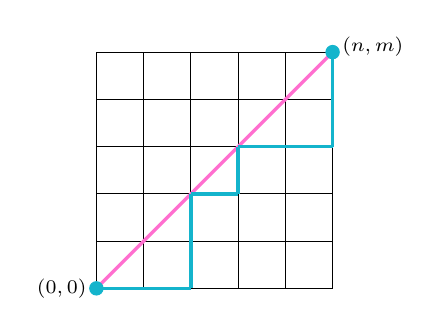
\begin{tikzpicture}[scale=0.6, bla node/.style={font=\scriptsize,draw=vhilight,text=vhilight,fill=vhilight}]
          \draw[step=1.0cm, thin, foreground] (0,0) grid (5,5);
          \draw[vhilight,very thick] (0,0) -- (5,5);
          \draw[hilight,fill] (0,0) circle[radius=4pt];
          \draw[hilight,fill] (5,5) circle[radius=4pt];
          \draw (0,0) node[anchor=east] {\scriptsize$(0,0)$};
          \draw (5,5) node[anchor=west,yshift=2pt] {\scriptsize$(n,m)$};

          \onslide<2->{
          \draw[hilight, very thick] (0,0) -- (2,0);
          \draw[hilight, very thick] (2,0) -- (2,2);
          \draw[hilight, very thick] (2,2) -- (3,2);
          \draw[hilight, very thick] (3,2) -- (3,3);
          \draw[hilight, very thick] (3,3) -- (5,3);
          \draw[hilight, very thick] (5,3) -- (5,5);
          }
        \end{tikzpicture}
      \end{figure}
    \end{column}
    \begin{column}{.6\textwidth}
      \bi
        \onslide<2->
        \item The number of paths from $(0,0)$ to $(n,m)$
          \[
            C_n = \frac{1}{n+1}\binom{2n}{n}
          \]
        \onslide<3->
        \item $C_n$ are known as Catalan numbers.
        \item Many problems involve solutions given by the Catalan numbers.
      \ei
    \end{column}
  \end{columns}
\end{frame}

\begin{frame}
  \bi
    \item Number of different ways $n+1$ factors can be completely parenthesized.
      \[
        ((ab)c)d\quad(a(bc))d\quad(ab)(cd)\quad a((bc)d)\quad a(b(cd))
      \]
    \onslide<2->
    \item Number of stack sortable permutations of length $n$.
    \onslide<3->
    \item Number of different triangulations convex polygon with $n+2$ sides
      \begin{figure}
        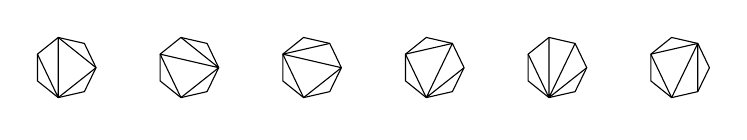
\begin{tikzpicture}[scale=0.4]
          \coordinate (A) at (-0.76,1.54);
          \coordinate (B) at (-0.76,0.69);
          \coordinate (C) at (-0.10,0.16);
          \coordinate (D) at (0.73,0.35);
          \coordinate (E) at (1.1,1.11);
          \coordinate (F) at (0.73,1.88);
          \coordinate (G) at (-0.10,2.07);

          \matrix[ampersand replacement=\&, column sep=0.8cm,row sep=0.5cm] {
            \slice{A/C,C/E,E/G,C/G}\&
            \slice{A/C,C/E,E/G,A/E}\&

            \slice{A/C,C/E,A/E,A/F}\&
            \slice{A/C,C/E,C/F,A/F}\&
            \slice{A/C,C/E,C/F,C/G}\&

            \slice{A/C,C/F,D/F,A/F}\\
          };
        \end{tikzpicture}
      \end{figure}
    \onslide<4->
    \item Number of full binary trees with $n+1$ leaves.
    \onslide<5->
    \item And aloot more.
  \ei
\end{frame}

\subsection{Fibonacci}
\begin{frame}
  The Fibonacci sequence is defined recursively as
  \begin{align*}
    &f_1 = 1\\
    &f_2 = 1\\
    &f_n = f_{n-1} + f_{n-2}
  \end{align*}
  \onslide<2->
  Already covered how to calculate $f_n$ in $O(N)$ time with dynamic programming.\\
  \onslide<3->
  But we can do even better.
\end{frame}

\subsection{Fibonacci as matrix}

\begin{frame}[fragile]
  \vspace{20pt}
  The Fibonacci sequence can be represented by a vectors
  \[
    \begin{pmatrix*}
      f_{n+2} \\
      f_{n+1}
    \end{pmatrix*}
    = 
    \begin{pmatrix*}
      1 & 1 \\
      1 & 0
    \end{pmatrix*}
    \begin{pmatrix*}
      f_{n+1} \\
      f_n
    \end{pmatrix*}
  \]
  \onslide<2->
  Or simply as a matrix
  \[
    \begin{pmatrix*}
      1 & 1 \\
      1 & 0
    \end{pmatrix*}^n =
    \begin{pmatrix*}
      f_{n+1} & f_n\\
      f_n & f_{n-1}
    \end{pmatrix*}
  \]
  \onslide<3->
  Using fast exponentiaton, we can calculate $f_n$ in $O(\log N)$ time.
\end{frame}

\begin{frame}
  \vspace{20pt}
  Any linear recurrence 
  \[
    a_n = c_1 a_{n-1} + c_2 a_{n-2} \ldots c_k a_{n-k}
  \]
  can be expressed in the same way
  \[
    \begin{pmatrix*}
      a_{n+1} \\
      a_{n} \\
      \vdots \\
      a_{n-k}
    \end{pmatrix*}
    =
    \begin{pmatrix}
      c_1 & c_2 & \ldots & c_k \\
      1 & 0 & \ldots & 0 \\
      \vdots & & \vdots \\
      0 & 0 & \ldots & 0 \\
    \end{pmatrix}
    \begin{pmatrix*}
      a_{n} \\
      a_{n-1} \\
      \vdots \\
      a_{n-k-1}
    \end{pmatrix*}
  \]
  \onslide<2->
  With a recurrence relation defined as a linear function of the $k$ preceding
  terms the running time will be $O(k^3 \log N)$.
\end{frame}

%%%%%%%%%%%%GAME THEORY%%%%%%%%%%%%%%%%%%%%%%%%%%%%%%%%%%%%%%%%%%%%%%%%%%%%%%%%%

\section{Game Theory}
\subsection{Game theory}
\begin{frame}
  \vspace{20pt}
  Game theory is the study of strategic decision making, but in competitive
  programming we are mostly interested in combinatorial games. \\
  \vspace{7pt}
  \onslide<2->
  %Game theory in competitive programming is mostly combinatorial games.
  Example:
  \bi
    \item There is a pile of $k$ matches.
    \item Player can remove $1$, $2$ or $3$ from the pile and alternate on moves.
    \item The player who removes the last match wins.
    \item There are two players, and the first player starts.
    \item Assuming that both players play perfectly, who wins?
  \ei
\end{frame}

\begin{frame}
  \vspace{10pt}
  We can analyse these types of games with \emph{backward induction}.\\ 
  \onslide<2->
  We call a state $N$-position if it is a winning state for the next player to
  move, and $P$-position if it is a winning position for the previous player.
  %Let $P$ denote a winning state for the previous player and $N$ denote a
  %winning state for the next player to move.
  \bi
    \item All terminal positions are $P$-positions.
    \item If every reachable state from the current one is a $N$-position then
      the current state is a $P$-position.
    \item If at least one $P$-position can be reached from the current one,
      then the current state is a $N$-position.
    \item A position is a $P$-position if all reachable states form the current
      one are $N$ position.
  \ei
\end{frame}

\begin{frame}
  \vspace{20pt}
  Let's analyse our previous game.
  \onslide<2->{
  \bi
    \item  The terminal position is a $P$-position.
    \onslide<3->{
  \item The positions reachable from the terminal positions are $N$-positions.}
    \onslide<4->{
  \item Position $4$ can only reach $N$-positions, therefore a $P$ position.}
    \onslide<5->{
  \item The next 3 positions can reach the $P$-position $4$, therefore they are $N$-positions.}
    \onslide<6->{
  \item And so on.}
  \ei
  \begin{center}
    \begin{tabular}{ c c c c c c c c c c c c c c c c c}
      $0$ & $1$ & $2$ & $3$ & $4$ & $5$ & $6$ & $7$ & $8$ & $9$ & $10$ & $11$ & $12$ & \ldots \\ \hline
      \onslide<2->{$P$} & \onslide<3->{$N$} &\onslide<3->{$N$}
      &\onslide<3->{$N$} & \onslide<4->{$P$}&\onslide<5->{$N$}
      &\onslide<5->{$N$} &\onslide<5->{$N$} &\onslide<6->{$P$}
      &\onslide<6->{$N$} &\onslide<6->{$N$} &\onslide<6->{$N$}
      &\onslide<6->{$P$} & \onslide<6->{\ldots}
    \end{tabular}
  \end{center}}
\end{frame}

\begin{frame}
  \vspace{40pt}
  We can see a clear pattern of the $N$ and $P$ positions in the previous game.
  -- Easy to prove that a position is $P$ if $x \equiv 0 \pmod{p}$.
  \onslide<2->
  \bi
    \item Many games can be analyzed this way.
    \item Not only one dimensional games.
    \onslide<3->
    \item What if there are $n$ piles instead of $1$?
    \onslide<4->
    \item What if we can remove $1$, $3$ or $4$?
  \ei
  \vspace{10pt}
\end{frame}

\subsection{The game called Nim}
\begin{frame}
  \vspace{40pt}
  \bi
    \item There are $n$ piles, each containing $x_i$ chips.
    \item Player can remove from exactly one pile, and can remove any number of chips.
    \item The player who removes the last match wins.
    \item There are two players, and the first player starts and they alternate on moves.
    \item Assuming that both players play perfectly, who wins?
  \ei
\end{frame}

\begin{frame}
  \vspace{40pt}
  Nim can be analyzed with $N$ and $P$ position.
  \bi
    \onslide<2->
    \item Not trivial to generalize over $n$ piles.
    \onslide<3->
    \item Luckily someone has already done that for us.
  \ei
  \vspace{10pt}
  \onslide<4->
  \emph{Buton's theorem} states that a position $(x_1, x_2, \ldots, x_n)$ in
  Nim is a $P$-position if and only if the xor over the number of chips is
  $0$. \\
  \onslide<5->
  \vspace{10pt}
  This theorem extends to other sums of combinatorial games!
\end{frame}

\begin{frame}[fragile]
  \vspace{20pt}
  Games can often also be viewed as graphs.
  \onslide<2->
  \bi
    \item Node for each state in the game.
    \item The edges are transitions from one state to the next.
  \ei
  \vspace{10pt}
  \onslide<3->
  Like the first subtraction game.
  \begin{figure}
    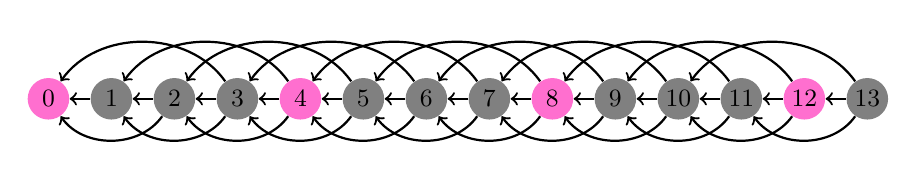
\begin{tikzpicture}[auto,scale=0.8]

      \node[vertex,color=vhilight] (0) at (0,0) {\color{foreground}0};
      \node[vertex] (1) at (1,0) {1};
      \node[vertex] (2) at (2,0) {2};
      \node[vertex] (3) at (3,0) {3};
      \node[vertex,color=vhilight] (4) at (4,0) {\color{foreground}4};
      \node[vertex] (5) at (5,0) {5};
      \node[vertex] (6) at (6,0) {6};
      \node[vertex] (7) at (7,0) {7};
      \node[vertex,color=vhilight] (8) at (8,0) {\color{foreground}8};
      \node[vertex] (9) at (9,0) {9};
      \node[vertex] (10) at (10,0) {10};
      \node[vertex] (11) at (11,0) {11};
      \node[vertex,color=vhilight] (12) at (12,0) {\color{foreground}12};
      \node[vertex] (13) at (13,0) {13};

      \path[dedge] (1) -- (0);

      \path[dedge] (2) edge[bend left=55] (0);
      \path[dedge] (2) -- (1);

      \path[dedge] (3) edge[bend right=55] (0);
      \path[dedge] (3) edge[bend left=55] (1);
      \path[dedge] (3) -- (2);

      \path[dedge] (4) edge[bend right=55] (1);
      \path[dedge] (4) edge[bend left=55] (2);
      \path[dedge] (4) -- (3);

      \path[dedge] (5) edge[bend right=55] (2);
      \path[dedge] (5) edge[bend left=55] (3);
      \path[dedge] (5) -- (4);

      \path[dedge] (6) edge[bend right=55] (3);
      \path[dedge] (6) edge[bend left=55] (4);
      \path[dedge] (6) -- (5);

      \path[dedge] (7) edge[bend right=55] (4);
      \path[dedge] (7) edge[bend left=55] (5);
      \path[dedge] (7) -- (6);

      \path[dedge] (8) edge[bend right=55] (5);
      \path[dedge] (8) edge[bend left=55] (6);
      \path[dedge] (8) -- (7);

      \path[dedge] (9) edge[bend right=55] (6);
      \path[dedge] (9) edge[bend left=55] (7);
      \path[dedge] (9) -- (8);

      \path[dedge] (10) edge[bend right=55] (7);
      \path[dedge] (10) edge[bend left=55] (8);
      \path[dedge] (10) -- (9);

      \path[dedge] (11) edge[bend right=55] (8);
      \path[dedge] (11) edge[bend left=55] (9);
      \path[dedge] (11) -- (10);

      \path[dedge] (12) edge[bend right=55] (9);
      \path[dedge] (12) edge[bend left=55] (10);
      \path[dedge] (12) -- (11);

      \path[dedge] (13) edge[bend right=55] (10);
      \path[dedge] (13) edge[bend left=55] (11);
      \path[dedge] (13) -- (12);

    \end{tikzpicture}
  \end{figure}
  We often denote the set of states(vertices) as $X$ instead of $V$ and edges as $F$ instead of $E$.
\end{frame}

\subsection{Sprague-Grundy}
\begin{frame}
  \vspace{30pt}
  Games can also be analysed with the \emph{Sprague-Grundy} function.
  \bi
    \item The \emph{Sprague-Grundy} function of a graph $(X,F)$, is a function $g$ defined on $X$ and taking non-negative integer values such that
      \[
        g(x) = \min\{n \geq\, :\, n \neq g(y) \}
      \]
    \onslide<2->
    \item The smallest non-negative integer among the Sprague-Grundy values of
      the followers of $x$ (states which $x$ has an edge to).
  \ei
\end{frame}

\begin{frame}
  \vspace{30pt}
  The smallest non-negative integer not among a set of non-negative integers is
  called the \textbf{minimal excludant}, or \textbf{mex}.\\
  \onslide<2->
  For example:
  \bi
    \item The minimal excludant of $\{0,1,2,5,6\}$ is $3$.
    \item The minimal excludant of $\{1,2,3,4,5\}$ is $0$.
  \ei
  \onslide<3->
  We can redefine the Sprague-Grundy function
  \[
    g(x) = \text{mex}\{g(y) \, : \, y \in F(x)\}
  \]
\end{frame}

\begin{frame}[fragile]
  \vspace{30pt}
  The graph of the previous game. \\
  \vspace{10pt}
  \onslide<2->{Adding the Sprague-Grundy value.}
  \begin{figure}
    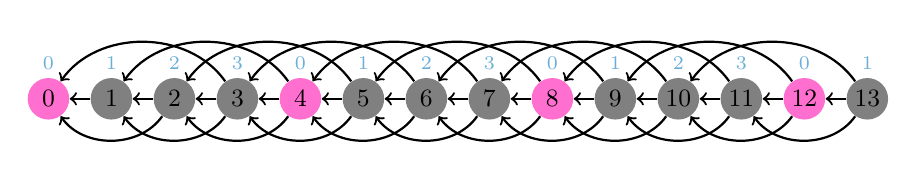
\begin{tikzpicture}[scale=0.8,auto]

      \node[vertex,color=vhilight] (0) at (0,0) {\color{foreground}0};
      \node[vertex] (1) at (1,0) {1};
      \node[vertex] (2) at (2,0) {2};
      \node[vertex] (3) at (3,0) {3};
      \node[vertex,color=vhilight] (4) at (4,0) {\color{foreground}4};
      \node[vertex] (5) at (5,0) {5};
      \node[vertex] (6) at (6,0) {6};
      \node[vertex] (7) at (7,0) {7};
      \node[vertex,color=vhilight] (8) at (8,0) {\color{foreground}8};
      \node[vertex] (9) at (9,0) {9};
      \node[vertex] (10) at (10,0) {10};
      \node[vertex] (11) at (11,0) {11};
      \node[vertex,color=vhilight] (12) at (12,0) {\color{foreground}12};
      \node[vertex] (13) at (13,0) {13};

      \path[dedge] (1) -- (0);

      \path[dedge] (2) edge[bend left=55] (0);
      \path[dedge] (2) -- (1);

      \path[dedge] (3) edge[bend right=55] (0);
      \path[dedge] (3) edge[bend left=55] (1);
      \path[dedge] (3) -- (2);

      \path[dedge] (4) edge[bend right=55] (1);
      \path[dedge] (4) edge[bend left=55] (2);
      \path[dedge] (4) -- (3);

      \path[dedge] (5) edge[bend right=55] (2);
      \path[dedge] (5) edge[bend left=55] (3);
      \path[dedge] (5) -- (4);

      \path[dedge] (6) edge[bend right=55] (3);
      \path[dedge] (6) edge[bend left=55] (4);
      \path[dedge] (6) -- (5);

      \path[dedge] (7) edge[bend right=55] (4);
      \path[dedge] (7) edge[bend left=55] (5);
      \path[dedge] (7) -- (6);

      \path[dedge] (8) edge[bend right=55] (5);
      \path[dedge] (8) edge[bend left=55] (6);
      \path[dedge] (8) -- (7);

      \path[dedge] (9) edge[bend right=55] (6);
      \path[dedge] (9) edge[bend left=55] (7);
      \path[dedge] (9) -- (8);

      \path[dedge] (10) edge[bend right=55] (7);
      \path[dedge] (10) edge[bend left=55] (8);
      \path[dedge] (10) -- (9);

      \path[dedge] (11) edge[bend right=55] (8);
      \path[dedge] (11) edge[bend left=55] (9);
      \path[dedge] (11) -- (10);

      \path[dedge] (12) edge[bend right=55] (9);
      \path[dedge] (12) edge[bend left=55] (10);
      \path[dedge] (12) -- (11);

      \path[dedge] (13) edge[bend right=55] (10);
      \path[dedge] (13) edge[bend left=55] (11);
      \path[dedge] (13) -- (12);

      \onslide<2->{
          \node[font=\scriptsize,shift={(0,0.45)},color=title] at (0) {0};
          \node[font=\scriptsize,shift={(0,0.45)},color=title] at (1) {1};
          \node[font=\scriptsize,shift={(0,0.45)},color=title] at (2) {2};
          \node[font=\scriptsize,shift={(0,0.45)},color=title] at (3) {3};
          \node[font=\scriptsize,shift={(0,0.45)},color=title] at (4) {0};
          \node[font=\scriptsize,shift={(0,0.45)},color=title] at (5) {1};
          \node[font=\scriptsize,shift={(0,0.45)},color=title] at (6) {2};
          \node[font=\scriptsize,shift={(0,0.45)},color=title] at (7) {3};
          \node[font=\scriptsize,shift={(0,0.45)},color=title] at (8) {0};
          \node[font=\scriptsize,shift={(0,0.45)},color=title] at (9) {1};
          \node[font=\scriptsize,shift={(0,0.45)},color=title] at (10) {2};
          \node[font=\scriptsize,shift={(0,0.45)},color=title] at (11) {3};
          \node[font=\scriptsize,shift={(0,0.45)},color=title] at (12) {0};
          \node[font=\scriptsize,shift={(0,0.45)},color=title] at (13) {1};
      }
    \end{tikzpicture}
  \end{figure}
  \onslide<3->
  Position $x$ is a $P$ position iff. $g(x) = 0$.
\end{frame}

\subsection{Sum of combinatorial games}
\begin{frame}
  \vspace{20pt}
  Back to Nim
  \bi
    \item Easy to see that for a position $x$ in Nim, $g(x) = x$.
    \onslide<2->
    \item What is the Sprague-Grundy value for multiple piles?
  \ei
  \onslide<3->
  If $g_i$ is the Sprague-Grundy function of $G_i$, $i = 1,2,\ldots,n$, then $G
  = G_1 + G_2 + \ldots + G_n$ has the Sprague-Grundy function
  \[
    g(x_1, x_2,\ldots,x_n) = g_1(x_1) \oplus g_2(x_2) \oplus \ldots \oplus g_n(x_n)
  \]
  \onslide<4->
  The sum of games can simply be thought of as the cartesian product of the
  positions, but each move consists of a move in one game. Just like Nim, where
  we can only remove chips from one pile.
\end{frame}

\begin{frame}
  \vspace{15pt}
  For example, if we have one pile which we can remove $1$,$2$ or $3$ and
  another one where we can remove any number of chips.
  \onslide<2->
  \bi
\item The Sprague-Grundy function of the first game is \[g_1(x) = x \pmod{4}\]
    \item The Sprague-Grundy function of the second game is \[g_2(x) = x\]
  \ei
  \onslide<3->
  What are the $P$ positions?
  \bi
    \onslide<4->
    \item Is $(7,5)$ a $P$ position?
      \[
        g_1(7) \oplus g_2(5) = 3 \oplus 5 = 6 \quad\quad\onslide<5->{\color{vhilight}\text{No}}
      \]
  \ei
\end{frame}

\begin{frame}{Applications}
  \vspace{20pt}
  Game theory is much more than just combinatorial game theory. \\
  \onslide<2->
  Applications:
  \bi
    \item Business
    \item Economics
    \item Sociology
    \item Psychology
    \item Many fields of mathematics, including computer science.
  \ei
  \onslide<3->
  \vspace{10pt}
  Take the Game Theory course if you want to know more.
\end{frame}

%%%%%%PROBABILITY THEORY%%%%%%%%%%%%%%%%%%%%%%%%%%%%%%%%%%%%%%%%%%%%%%%%%%%%%%%%

%\section{Probability theory}
%\subsection{Probability theory}

%\begin{frame}
  %Probability theory.
%\end{frame}

%%%%%%%BIG INTEGER%%%%%%%%%%%%%%%%%%%%%%%%%%%%%%%%%%%%%%%%%%%%%%%%%%%%%%%%%%%%%

%\section{Big integer}
%\subsection{Big integer}

%\begin{frame}
  %\vspace{30pt}
  %Sometimes we need integer types that do not fit in $64$ bits.
  %\onslide<2->
  %\bi
    %\item In Java there is the \texttt{BigInteger} class.
    %\onslide<3->
    %\item Allows arbitrary sized integers.
    %\onslide<4->
    %\item Also no problem for Python and some other programming languages.
  %\ei
  %\vspace{10pt}
  %What about \texttt{C/C++}?
  %\bi
    %\item We can write our own \texttt{BigInteger} type!
  %\ei
%\end{frame}

%\begin{frame}[fragile]
  %The main idea behind our implementation
  %\onslide<2->
  %\bi
    %\item Number is represented as an array of integers.
    %\onslide<3->
    %\item Each integer in the array represents some fixed number of digits of the big integer.
    %\onslide<4->
    %\item You can think of it as storing the number in base $10^k$
    %\onslide<5->
    %\item When doing arithmetic, we carry value up or down while iterating through the digits.
  %\ei
  %\begin{minted}{cpp}
%struct BigInteger {
    %int sign;
    %vector<unsigned int> data;
    %static const int dcnt = 9;
    %static const unsigned int radix = 1000000000U;
    %...
%};
  %\end{minted}
%\end{frame}

%\subsection{Addition and subtraction}
%\begin{frame}[fragile]
  %\vspace{20pt}
  %Addition is performed like in primary school.
  %\onslide<2->
  %\bi
    %\item Starting from least significant digits, add the two digits and the carry.
    %\onslide<3->
    %\item If the value exceeds the base, divide by the base.
    %\onslide<4->
    %\item The carry takes the quotient and the remainder stays in that digit.
  %\ei
  %\begin{figure}
    %\begin{tabular}{c c c c c}
       %&\onslide<9->{$1$} &\onslide<7->{$1$} & & \\
      %& & $2$ & $3$ & $7$ \\
      %$+$ & $1$ & $8$ & $9$ & $2$ \\\hline
      %& \onslide<10->{$2$} & \onslide<8->{$1$} & \onslide<6->{$2$} & \onslide<5->{$9$}
    %\end{tabular}
  %\end{figure}
%\end{frame}

%\begin{frame}[fragile]
  %\vspace{20pt}
  %Subtraction is performed very much like addition.
  %\onslide<2->
  %\bi
    %\item Starting from the least significant digits, subtract the lower digit from the upper.
    %\onslide<3->
    %\item If the outcome is negative, we \emph{borrow} from the next digit,
      %like a negative carry and finally we add the negative value to the base and store in the digit.
  %\ei
  %\begin{figure}
    %\begin{tabular}{c c c c c}
      %\onslide<5->{$-$} & \onslide<8->{$1$} & &\onslide<5->{$1$} & \\
      %& $1$ & $8$ & $9$ & $2$ \\
      %$-$ & & $9$ & $3$ & $7$ \\\hline
      %& \onslide<9>{$0$}  & \onslide<7->{$8$} & \onslide<6->{$5$} & \onslide<4->{$5$}
    %\end{tabular}
  %\end{figure}
%\end{frame}

%\begin{frame}[fragile]
  %\begin{minted}[fontsize=\small]{cpp}
%BigInteger operator+(const BigInteger& b){
  %...
  %BigInteger c;
  %unsigned long long carry = 0;
  %for (int i = 0; i < size() || i < b.size() || carry; i++) {
      %if(i < size())
          %carry += data[i];
      %if(i < b.size())
          %carry += b.data[i];
      %c.data.push_back(carry % BigInteger::radix);
      %carry /= BigInteger::radix;
  %}
  %return c.normalize(sign);
%}
  %\end{minted}
%\end{frame}

%\begin{frame}[fragile]
  %\begin{minted}[fontsize=\small]{cpp}
%BigInteger operator-(const BigInteger& b) {
  %...
  %BigInteger c;
  %long long borrow = 0;
  %for (int i = 0; i < size(); i++) {
      %borrow = data[i] - borrow;
      %if(i < b.size())
          %borrow -= b.data[i];
      %if(borrow < 0)
          %c.data.push_back(BigInteger::radix + borrow);
      %else
          %c.data.push_back(borrow);
      %borrow = borrow < 0 ? 1 : 0;
  %}
  %return c.normalize(sign);
%}
  %\end{minted}
%\end{frame}

%CHECK : Modular Arithmetic
% - Identities, ring over modulus
%CHECK : GCD, LCM, Extended Euclidean
%CHECK : Modular inverse
%CHECK : Modular exponentiation, repeated squaring already covered
%CHECK : Chinese remainder theorem
%CHECK : Primality testing
%CHECK : Sieve
%CHECK : Factoring
%CHECK: Factor identities, factor sums, count, totient phi,

% COMBINATORICS
%CHECK: Binomial coefficients
%CHECK: Counting identities
% - Fibonacci, Zeckendorff's Theorem
% - Binomial(Identities)
% - Factorial(Identities)
% - Catalan(Identities)
% - Stirling

% MATRIX TRICKS
%CHECK: Linear recurrences
% - Matrix multiplication
%TODO: Adjacency matrix
% - Number of paths, power of matrix
%
% GAME THEORY
%CHECK : Nim
%CHECK : N & P states
%CHECK : Sprague-Grundy
%
% PROBABILITY THEORY
%TODO: Probability theory basics
%TODO: Bernoulli distribution
%TODO: Something discrete?
%
%NOT: Java BigInteger
% - How to implement
%
%MAYBE: Numerical integration(Riemann sum), system of linear equations, linear Diophantine, cycle finding
%

\end{document}

